\documentclass[1p]{elsarticle_modified}
%\bibliographystyle{elsarticle-num}

%\usepackage[colorlinks]{hyperref}
%\usepackage{abbrmath_seonhwa} %\Abb, \Ascr, \Acal ,\Abf, \Afrak
\usepackage{amsfonts}
\usepackage{amssymb}
\usepackage{amsmath}
\usepackage{amsthm}
\usepackage{scalefnt}
\usepackage{amsbsy}
\usepackage{kotex}
\usepackage{caption}
\usepackage{subfig}
\usepackage{color}
\usepackage{graphicx}
\usepackage{xcolor} %% white, black, red, green, blue, cyan, magenta, yellow
\usepackage{float}
\usepackage{setspace}
\usepackage{hyperref}

\usepackage{tikz}
\usetikzlibrary{arrows}

\usepackage{multirow}
\usepackage{array} % fixed length table
\usepackage{hhline}

%%%%%%%%%%%%%%%%%%%%%
\makeatletter
\renewcommand*\env@matrix[1][\arraystretch]{%
	\edef\arraystretch{#1}%
	\hskip -\arraycolsep
	\let\@ifnextchar\new@ifnextchar
	\array{*\c@MaxMatrixCols c}}
\makeatother %https://tex.stackexchange.com/questions/14071/how-can-i-increase-the-line-spacing-in-a-matrix
%%%%%%%%%%%%%%%

\usepackage[normalem]{ulem}

\newcommand{\msout}[1]{\ifmmode\text{\sout{\ensuremath{#1}}}\else\sout{#1}\fi}
%SOURCE: \msout is \stkout macro in https://tex.stackexchange.com/questions/20609/strikeout-in-math-mode

\newcommand{\cancel}[1]{
	\ifmmode
	{\color{red}\msout{#1}}
	\else
	{\color{red}\sout{#1}}
	\fi
}

\newcommand{\add}[1]{
	{\color{blue}\uwave{#1}}
}

\newcommand{\replace}[2]{
	\ifmmode
	{\color{red}\msout{#1}}{\color{blue}\uwave{#2}}
	\else
	{\color{red}\sout{#1}}{\color{blue}\uwave{#2}}
	\fi
}

\newcommand{\Sol}{\mathcal{S}} %segment
\newcommand{\D}{D} %diagram
\newcommand{\A}{\mathcal{A}} %arc


%%%%%%%%%%%%%%%%%%%%%%%%%%%%%5 test

\def\sl{\operatorname{\textup{SL}}(2,\Cbb)}
\def\psl{\operatorname{\textup{PSL}}(2,\Cbb)}
\def\quan{\mkern 1mu \triangleright \mkern 1mu}

\theoremstyle{definition}
\newtheorem{thm}{Theorem}[section]
\newtheorem{prop}[thm]{Proposition}
\newtheorem{lem}[thm]{Lemma}
\newtheorem{ques}[thm]{Question}
\newtheorem{cor}[thm]{Corollary}
\newtheorem{defn}[thm]{Definition}
\newtheorem{exam}[thm]{Example}
\newtheorem{rmk}[thm]{Remark}
\newtheorem{alg}[thm]{Algorithm}

\newcommand{\I}{\sqrt{-1}}
\begin{document}

%\begin{frontmatter}
%
%\title{Boundary parabolic representations of knots up to 8 crossings}
%
%%% Group authors per affiliation:
%\author{Yunhi Cho} 
%\address{Department of Mathematics, University of Seoul, Seoul, Korea}
%\ead{yhcho@uos.ac.kr}
%
%
%\author{Seonhwa Kim} %\fnref{s_kim}}
%\address{Center for Geometry and Physics, Institute for Basic Science, Pohang, 37673, Korea}
%\ead{ryeona17@ibs.re.kr}
%
%\author{Hyuk Kim}
%\address{Department of Mathematical Sciences, Seoul National University, Seoul 08826, Korea}
%\ead{hyukkim@snu.ac.kr}
%
%\author{Seokbeom Yoon}
%\address{Department of Mathematical Sciences, Seoul National University, Seoul, 08826,  Korea}
%\ead{sbyoon15@snu.ac.kr}
%
%\begin{abstract}
%We find all boundary parabolic representation of knots up to 8 crossings.
%
%\end{abstract}
%\begin{keyword}
%    \MSC[2010] 57M25 
%\end{keyword}
%
%\end{frontmatter}

%\linenumbers
%\tableofcontents
%
\newcommand\colored[1]{\textcolor{white}{\rule[-0.35ex]{0.8em}{1.4ex}}\kern-0.8em\color{red} #1}%
%\newcommand\colored[1]{\textcolor{white}{ #1}\kern-2.17ex	\textcolor{white}{ #1}\kern-1.81ex	\textcolor{white}{ #1}\kern-2.15ex\color{red}#1	}

{\Large $\underline{12a_{0278}~(K12a_{0278})}$}

\setlength{\tabcolsep}{10pt}
\renewcommand{\arraystretch}{1.6}
\vspace{1cm}\begin{tabular}{m{100pt}>{\centering\arraybackslash}m{274pt}}
\multirow{5}{120pt}{
	\centering
	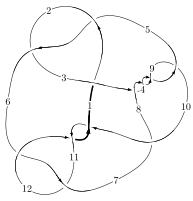
\includegraphics[width=112pt]{../../../GIT/diagram.site/Diagrams/png/1079_12a_0278.png}\\
\ \ \ A knot diagram\footnotemark}&
\allowdisplaybreaks
\textbf{Linearized knot diagam} \\
\cline{2-2}
 &
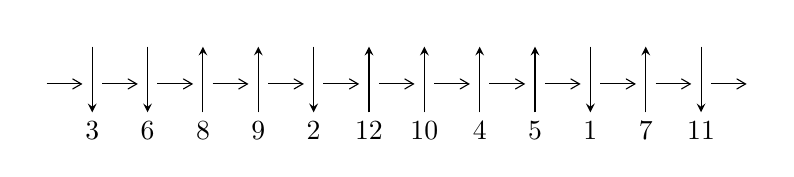
\begin{tikzpicture}[x=20pt, y=17pt]
	% nodes
	\node (C0) at (0, 0) {};
	\node (C1) at (1, 0) {};
	\node (C1U) at (1, +1) {};
	\node (C1D) at (1, -1) {3};

	\node (C2) at (2, 0) {};
	\node (C2U) at (2, +1) {};
	\node (C2D) at (2, -1) {6};

	\node (C3) at (3, 0) {};
	\node (C3U) at (3, +1) {};
	\node (C3D) at (3, -1) {8};

	\node (C4) at (4, 0) {};
	\node (C4U) at (4, +1) {};
	\node (C4D) at (4, -1) {9};

	\node (C5) at (5, 0) {};
	\node (C5U) at (5, +1) {};
	\node (C5D) at (5, -1) {2};

	\node (C6) at (6, 0) {};
	\node (C6U) at (6, +1) {};
	\node (C6D) at (6, -1) {12};

	\node (C7) at (7, 0) {};
	\node (C7U) at (7, +1) {};
	\node (C7D) at (7, -1) {10};

	\node (C8) at (8, 0) {};
	\node (C8U) at (8, +1) {};
	\node (C8D) at (8, -1) {4};

	\node (C9) at (9, 0) {};
	\node (C9U) at (9, +1) {};
	\node (C9D) at (9, -1) {5};

	\node (C10) at (10, 0) {};
	\node (C10U) at (10, +1) {};
	\node (C10D) at (10, -1) {1};

	\node (C11) at (11, 0) {};
	\node (C11U) at (11, +1) {};
	\node (C11D) at (11, -1) {7};

	\node (C12) at (12, 0) {};
	\node (C12U) at (12, +1) {};
	\node (C12D) at (12, -1) {11};
	\node (C13) at (13, 0) {};

	% arrows
	\draw[->,>={angle 60}]
	(C0) edge (C1) (C1) edge (C2) (C2) edge (C3) (C3) edge (C4) (C4) edge (C5) (C5) edge (C6) (C6) edge (C7) (C7) edge (C8) (C8) edge (C9) (C9) edge (C10) (C10) edge (C11) (C11) edge (C12) (C12) edge (C13) ;	\draw[->,>=stealth]
	(C1U) edge (C1D) (C2U) edge (C2D) (C3D) edge (C3U) (C4D) edge (C4U) (C5U) edge (C5D) (C6D) edge (C6U) (C7D) edge (C7U) (C8D) edge (C8U) (C9D) edge (C9U) (C10U) edge (C10D) (C11D) edge (C11U) (C12U) edge (C12D) ;
	\end{tikzpicture} \\
\hhline{~~} \\& 
\textbf{Solving Sequence} \\ \cline{2-2} 
 &
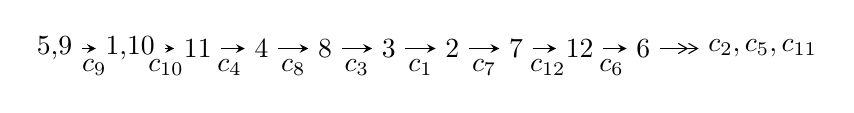
\begin{tikzpicture}[x=23pt, y=7pt]
	% node
	\node (A0) at (-1/8, 0) {5,9};
	\node (A1) at (17/16, 0) {1,10};
	\node (A2) at (17/8, 0) {11};
	\node (A3) at (25/8, 0) {4};
	\node (A4) at (33/8, 0) {8};
	\node (A5) at (41/8, 0) {3};
	\node (A6) at (49/8, 0) {2};
	\node (A7) at (57/8, 0) {7};
	\node (A8) at (65/8, 0) {12};
	\node (A9) at (73/8, 0) {6};
	\node (C1) at (1/2, -1) {$c_{9}$};
	\node (C2) at (13/8, -1) {$c_{10}$};
	\node (C3) at (21/8, -1) {$c_{4}$};
	\node (C4) at (29/8, -1) {$c_{8}$};
	\node (C5) at (37/8, -1) {$c_{3}$};
	\node (C6) at (45/8, -1) {$c_{1}$};
	\node (C7) at (53/8, -1) {$c_{7}$};
	\node (C8) at (61/8, -1) {$c_{12}$};
	\node (C9) at (69/8, -1) {$c_{6}$};
	\node (A10) at (11, 0) {$c_{2},c_{5},c_{11}$};

	% edge
	\draw[->,>=stealth]	
	(A0) edge (A1) (A1) edge (A2) (A2) edge (A3) (A3) edge (A4) (A4) edge (A5) (A5) edge (A6) (A6) edge (A7) (A7) edge (A8) (A8) edge (A9) ;
	\draw[->>,>={angle 60}]	
	(A9) edge (A10);
\end{tikzpicture} \\ 

\end{tabular} \\

\footnotetext{
The image of knot diagram is generated by the software ``\textbf{Draw programme}" developed by Andrew Bartholomew(\url{http://www.layer8.co.uk/maths/draw/index.htm\#Running-draw}), where we modified some parts for our purpose(\url{https://github.com/CATsTAILs/LinksPainter}).
}\phantom \\ \newline 
\centering \textbf{Ideals for irreducible components\footnotemark of $X_{\text{par}}$} 
 
\begin{align*}
I^u_{1}&=\langle 
9.38441\times10^{39} u^{74}+5.67453\times10^{39} u^{73}+\cdots+1.90771\times10^{40} b-5.20911\times10^{40},\\
\phantom{I^u_{1}}&\phantom{= \langle  }-1.62029\times10^{40} u^{74}-8.80257\times10^{39} u^{73}+\cdots+1.90771\times10^{40} a+1.14013\times10^{41},\;u^{75}+u^{74}+\cdots-12 u-4\rangle \\
I^u_{2}&=\langle 
b^2-2 b u- b+u+3,\;2 a+u,\;u^2-2\rangle \\
\\
I^v_{1}&=\langle 
a,\;b- v-1,\;v^2+v+1\rangle \\
\end{align*}
\raggedright * 3 irreducible components of $\dim_{\mathbb{C}}=0$, with total 81 representations.\\
\footnotetext{All coefficients of polynomials are rational numbers. But the coefficients are sometimes approximated in decimal forms when there is not enough margin.}
\newpage
\renewcommand{\arraystretch}{1}
\centering \section*{I. $I^u_{1}= \langle 9.38\times10^{39} u^{74}+5.67\times10^{39} u^{73}+\cdots+1.91\times10^{40} b-5.21\times10^{40},\;-1.62\times10^{40} u^{74}-8.80\times10^{39} u^{73}+\cdots+1.91\times10^{40} a+1.14\times10^{41},\;u^{75}+u^{74}+\cdots-12 u-4 \rangle$}
\flushleft \textbf{(i) Arc colorings}\\
\begin{tabular}{m{7pt} m{180pt} m{7pt} m{180pt} }
\flushright $a_{5}=$&$\begin{pmatrix}0\\u\end{pmatrix}$ \\
\flushright $a_{9}=$&$\begin{pmatrix}1\\0\end{pmatrix}$ \\
\flushright $a_{1}=$&$\begin{pmatrix}0.849339 u^{74}+0.461421 u^{73}+\cdots-10.4833 u-5.97644\\-0.491921 u^{74}-0.297453 u^{73}+\cdots+0.593748 u+2.73056\end{pmatrix}$ \\
\flushright $a_{10}=$&$\begin{pmatrix}1\\- u^2\end{pmatrix}$ \\
\flushright $a_{11}=$&$\begin{pmatrix}0.524536 u^{74}-0.696711 u^{73}+\cdots-8.34076 u-5.63903\\-1.23043 u^{74}+1.30629 u^{73}+\cdots+12.6838 u+6.35323\end{pmatrix}$ \\
\flushright $a_{4}=$&$\begin{pmatrix}- u\\u\end{pmatrix}$ \\
\flushright $a_{8}=$&$\begin{pmatrix}- u^2+1\\u^2\end{pmatrix}$ \\
\flushright $a_{3}=$&$\begin{pmatrix}u^3-2 u\\- u^3+u\end{pmatrix}$ \\
\flushright $a_{2}=$&$\begin{pmatrix}0.871842 u^{74}-0.0410241 u^{73}+\cdots-10.2878 u-6.19131\\-0.374527 u^{74}+0.413670 u^{73}+\cdots+1.18849 u+2.97556\end{pmatrix}$ \\
\flushright $a_{7}=$&$\begin{pmatrix}u^4-3 u^2+1\\- u^6+2 u^4+u^2\end{pmatrix}$ \\
\flushright $a_{12}=$&$\begin{pmatrix}0.519955 u^{74}-0.395542 u^{73}+\cdots-8.23310 u-4.93826\\-1.16106 u^{74}+0.963015 u^{73}+\cdots+11.8087 u+6.08819\end{pmatrix}$ \\
\flushright $a_{6}=$&$\begin{pmatrix}-0.174957 u^{74}-0.182489 u^{73}+\cdots-8.40404 u+0.258482\\0.672272 u^{74}+0.555135 u^{73}+\cdots-0.695264 u-3.47423\end{pmatrix}$\\&\end{tabular}
\flushleft \textbf{(ii) Obstruction class $= -1$}\\~\\
\flushleft \textbf{(iii) Cusp Shapes $= -2.15821 u^{74}+0.754780 u^{73}+\cdots+41.7200 u+28.2560$}\\~\\
\newpage\renewcommand{\arraystretch}{1}
\flushleft \textbf{(iv) u-Polynomials at the component}\newline \\
\begin{tabular}{m{50pt}|m{274pt}}
Crossings & \hspace{64pt}u-Polynomials at each crossing \\
\hline $$\begin{aligned}c_{1}\end{aligned}$$&$\begin{aligned}
&u^{75}+39 u^{74}+\cdots+417 u+49
\end{aligned}$\\
\hline $$\begin{aligned}c_{2},c_{5}\end{aligned}$$&$\begin{aligned}
&u^{75}+3 u^{74}+\cdots-9 u-7
\end{aligned}$\\
\hline $$\begin{aligned}c_{3},c_{4},c_{8}\\c_{9}\end{aligned}$$&$\begin{aligned}
&u^{75}+u^{74}+\cdots-12 u-4
\end{aligned}$\\
\hline $$\begin{aligned}c_{6},c_{11}\end{aligned}$$&$\begin{aligned}
&u^{75}-2 u^{74}+\cdots+6 u+1
\end{aligned}$\\
\hline $$\begin{aligned}c_{7}\end{aligned}$$&$\begin{aligned}
&u^{75}+15 u^{74}+\cdots+11264 u+1792
\end{aligned}$\\
\hline $$\begin{aligned}c_{10},c_{12}\end{aligned}$$&$\begin{aligned}
&u^{75}+26 u^{74}+\cdots+40 u-1
\end{aligned}$\\
\hline
\end{tabular}\\~\\
\newpage\renewcommand{\arraystretch}{1}
\flushleft \textbf{(v) Riley Polynomials at the component}\newline \\
\begin{tabular}{m{50pt}|m{274pt}}
Crossings & \hspace{64pt}Riley Polynomials at each crossing \\
\hline $$\begin{aligned}c_{1}\end{aligned}$$&$\begin{aligned}
&y^{75}+y^{74}+\cdots-65623 y-2401
\end{aligned}$\\
\hline $$\begin{aligned}c_{2},c_{5}\end{aligned}$$&$\begin{aligned}
&y^{75}-39 y^{74}+\cdots+417 y-49
\end{aligned}$\\
\hline $$\begin{aligned}c_{3},c_{4},c_{8}\\c_{9}\end{aligned}$$&$\begin{aligned}
&y^{75}-85 y^{74}+\cdots+272 y-16
\end{aligned}$\\
\hline $$\begin{aligned}c_{6},c_{11}\end{aligned}$$&$\begin{aligned}
&y^{75}+26 y^{74}+\cdots+40 y-1
\end{aligned}$\\
\hline $$\begin{aligned}c_{7}\end{aligned}$$&$\begin{aligned}
&y^{75}+19 y^{74}+\cdots+128483328 y-3211264
\end{aligned}$\\
\hline $$\begin{aligned}c_{10},c_{12}\end{aligned}$$&$\begin{aligned}
&y^{75}+50 y^{74}+\cdots+1936 y-1
\end{aligned}$\\
\hline
\end{tabular}\\~\\
\newpage\flushleft \textbf{(vi) Complex Volumes and Cusp Shapes}
$$\begin{array}{c|c|c}  
\text{Solutions to }I^u_{1}& \I (\text{vol} + \sqrt{-1}CS) & \text{Cusp shape}\\
 \hline 
\begin{aligned}
u &= \phantom{-}0.992360 + 0.148515 I \\
a &= \phantom{-}0.576542 + 0.197096 I \\
b &= -0.309129 + 0.852785 I\end{aligned}
 & \phantom{-}4.89966 - 0.48043 I & \phantom{-0.000000 } 0 \\ \hline\begin{aligned}
u &= \phantom{-}0.992360 - 0.148515 I \\
a &= \phantom{-}0.576542 - 0.197096 I \\
b &= -0.309129 - 0.852785 I\end{aligned}
 & \phantom{-}4.89966 + 0.48043 I & \phantom{-0.000000 } 0 \\ \hline\begin{aligned}
u &= -0.931734 + 0.252335 I \\
a &= -0.485930 + 0.342374 I \\
b &= \phantom{-}0.456955 + 0.767589 I\end{aligned}
 & \phantom{-}4.81883 - 5.04031 I & \phantom{-0.000000 } 0 \\ \hline\begin{aligned}
u &= -0.931734 - 0.252335 I \\
a &= -0.485930 - 0.342374 I \\
b &= \phantom{-}0.456955 - 0.767589 I\end{aligned}
 & \phantom{-}4.81883 + 5.04031 I & \phantom{-0.000000 } 0 \\ \hline\begin{aligned}
u &= \phantom{-}0.653012 + 0.614677 I \\
a &= -2.17237 + 0.30058 I \\
b &= \phantom{-}0.915870 + 0.280175 I\end{aligned}
 & -0.19940 + 12.18710 I & \phantom{-0.000000 } 0 \\ \hline\begin{aligned}
u &= \phantom{-}0.653012 - 0.614677 I \\
a &= -2.17237 - 0.30058 I \\
b &= \phantom{-}0.915870 - 0.280175 I\end{aligned}
 & -0.19940 - 12.18710 I & \phantom{-0.000000 } 0 \\ \hline\begin{aligned}
u &= -0.665614 + 0.580959 I \\
a &= \phantom{-}1.80487 + 0.31047 I \\
b &= -0.671344 + 0.328501 I\end{aligned}
 & \phantom{-}0.97505 - 6.50542 I & \phantom{-0.000000 } 0 \\ \hline\begin{aligned}
u &= -0.665614 - 0.580959 I \\
a &= \phantom{-}1.80487 - 0.31047 I \\
b &= -0.671344 - 0.328501 I\end{aligned}
 & \phantom{-}0.97505 + 6.50542 I & \phantom{-0.000000 } 0 \\ \hline\begin{aligned}
u &= -0.675215 + 0.522999 I \\
a &= -1.99689 + 0.08186 I \\
b &= \phantom{-}0.802298 - 0.038855 I\end{aligned}
 & \phantom{-}2.37245 - 7.04723 I & \phantom{-0.000000 -}0. + 7.05593 I \\ \hline\begin{aligned}
u &= -0.675215 - 0.522999 I \\
a &= -1.99689 - 0.08186 I \\
b &= \phantom{-}0.802298 + 0.038855 I\end{aligned}
 & \phantom{-}2.37245 + 7.04723 I & \phantom{-0.000000 } 0. - 7.05593 I\\
 \hline 
 \end{array}$$\newpage$$\begin{array}{c|c|c}  
\text{Solutions to }I^u_{1}& \I (\text{vol} + \sqrt{-1}CS) & \text{Cusp shape}\\
 \hline 
\begin{aligned}
u &= \phantom{-}0.697751 + 0.462610 I \\
a &= \phantom{-}1.71652 - 0.07976 I \\
b &= -0.612037 - 0.027947 I\end{aligned}
 & \phantom{-}3.26431 + 1.50095 I & \phantom{-}7.89789 - 1.80538 I \\ \hline\begin{aligned}
u &= \phantom{-}0.697751 - 0.462610 I \\
a &= \phantom{-}1.71652 + 0.07976 I \\
b &= -0.612037 + 0.027947 I\end{aligned}
 & \phantom{-}3.26431 - 1.50095 I & \phantom{-}7.89789 + 1.80538 I \\ \hline\begin{aligned}
u &= \phantom{-}0.567607 + 0.560344 I \\
a &= -1.81116 - 0.63783 I \\
b &= \phantom{-}0.795511 + 0.950961 I\end{aligned}
 & -5.29697 + 5.95713 I & -3.09818 - 7.38755 I \\ \hline\begin{aligned}
u &= \phantom{-}0.567607 - 0.560344 I \\
a &= -1.81116 + 0.63783 I \\
b &= \phantom{-}0.795511 - 0.950961 I\end{aligned}
 & -5.29697 - 5.95713 I & -3.09818 + 7.38755 I \\ \hline\begin{aligned}
u &= \phantom{-}0.323852 + 0.694398 I \\
a &= -0.48580 - 1.64617 I \\
b &= -0.386203 + 0.980438 I\end{aligned}
 & -1.18225 - 7.78836 I & \phantom{-}0.62681 + 5.55340 I \\ \hline\begin{aligned}
u &= \phantom{-}0.323852 - 0.694398 I \\
a &= -0.48580 + 1.64617 I \\
b &= -0.386203 - 0.980438 I\end{aligned}
 & -1.18225 + 7.78836 I & \phantom{-}0.62681 - 5.55340 I \\ \hline\begin{aligned}
u &= -0.591460 + 0.442465 I \\
a &= \phantom{-}0.851460 - 0.535667 I \\
b &= -0.167713 + 0.970251 I\end{aligned}
 & -0.68077 - 3.94349 I & \phantom{-}4.08468 + 7.42217 I \\ \hline\begin{aligned}
u &= -0.591460 - 0.442465 I \\
a &= \phantom{-}0.851460 + 0.535667 I \\
b &= -0.167713 - 0.970251 I\end{aligned}
 & -0.68077 + 3.94349 I & \phantom{-}4.08468 - 7.42217 I \\ \hline\begin{aligned}
u &= -0.282851 + 0.667116 I \\
a &= \phantom{-}0.407429 - 1.153780 I \\
b &= \phantom{-}0.460517 + 0.731193 I\end{aligned}
 & -0.16240 + 2.29905 I & \phantom{-}2.31301 - 0.75455 I \\ \hline\begin{aligned}
u &= -0.282851 - 0.667116 I \\
a &= \phantom{-}0.407429 + 1.153780 I \\
b &= \phantom{-}0.460517 - 0.731193 I\end{aligned}
 & -0.16240 - 2.29905 I & \phantom{-}2.31301 + 0.75455 I\\
 \hline 
 \end{array}$$\newpage$$\begin{array}{c|c|c}  
\text{Solutions to }I^u_{1}& \I (\text{vol} + \sqrt{-1}CS) & \text{Cusp shape}\\
 \hline 
\begin{aligned}
u &= \phantom{-}0.399552 + 0.588174 I \\
a &= -1.69508 - 1.30618 I \\
b &= \phantom{-}0.152200 + 0.661165 I\end{aligned}
 & -5.79484 - 2.02438 I & -5.06771 + 0.43859 I \\ \hline\begin{aligned}
u &= \phantom{-}0.399552 - 0.588174 I \\
a &= -1.69508 + 1.30618 I \\
b &= \phantom{-}0.152200 - 0.661165 I\end{aligned}
 & -5.79484 + 2.02438 I & -5.06771 - 0.43859 I \\ \hline\begin{aligned}
u &= \phantom{-}1.287660 + 0.137546 I \\
a &= \phantom{-}0.108222 + 0.102118 I \\
b &= -0.041567 - 1.232660 I\end{aligned}
 & \phantom{-}4.69216 + 0.68186 I & \phantom{-0.000000 } 0 \\ \hline\begin{aligned}
u &= \phantom{-}1.287660 - 0.137546 I \\
a &= \phantom{-}0.108222 - 0.102118 I \\
b &= -0.041567 + 1.232660 I\end{aligned}
 & \phantom{-}4.69216 - 0.68186 I & \phantom{-0.000000 } 0 \\ \hline\begin{aligned}
u &= -0.477179 + 0.487322 I \\
a &= -1.37904 + 0.78397 I \\
b &= \phantom{-}0.597926 - 0.495834 I\end{aligned}
 & -2.38002 - 1.71377 I & -0.33796 + 4.28154 I \\ \hline\begin{aligned}
u &= -0.477179 - 0.487322 I \\
a &= -1.37904 - 0.78397 I \\
b &= \phantom{-}0.597926 + 0.495834 I\end{aligned}
 & -2.38002 + 1.71377 I & -0.33796 - 4.28154 I \\ \hline\begin{aligned}
u &= \phantom{-}0.511035 + 0.444098 I \\
a &= -2.87952 - 0.72570 I \\
b &= \phantom{-}0.418047 + 0.120094 I\end{aligned}
 & -2.37090 + 3.74638 I & \phantom{-}0.22703 - 6.74943 I \\ \hline\begin{aligned}
u &= \phantom{-}0.511035 - 0.444098 I \\
a &= -2.87952 + 0.72570 I \\
b &= \phantom{-}0.418047 - 0.120094 I\end{aligned}
 & -2.37090 - 3.74638 I & \phantom{-}0.22703 + 6.74943 I \\ \hline\begin{aligned}
u &= \phantom{-}0.473672 + 0.440581 I \\
a &= -0.80128 - 1.37475 I \\
b &= \phantom{-}0.17379 + 1.52146 I\end{aligned}
 & -2.48507 - 0.60256 I & -0.45284 - 3.01495 I \\ \hline\begin{aligned}
u &= \phantom{-}0.473672 - 0.440581 I \\
a &= -0.80128 + 1.37475 I \\
b &= \phantom{-}0.17379 - 1.52146 I\end{aligned}
 & -2.48507 + 0.60256 I & -0.45284 + 3.01495 I\\
 \hline 
 \end{array}$$\newpage$$\begin{array}{c|c|c}  
\text{Solutions to }I^u_{1}& \I (\text{vol} + \sqrt{-1}CS) & \text{Cusp shape}\\
 \hline 
\begin{aligned}
u &= -1.342850 + 0.195956 I \\
a &= \phantom{-}0.162252 + 0.343427 I \\
b &= -0.00168 - 1.80697 I\end{aligned}
 & \phantom{-}4.05099 + 4.57027 I & \phantom{-0.000000 } 0 \\ \hline\begin{aligned}
u &= -1.342850 - 0.195956 I \\
a &= \phantom{-}0.162252 - 0.343427 I \\
b &= -0.00168 + 1.80697 I\end{aligned}
 & \phantom{-}4.05099 - 4.57027 I & \phantom{-0.000000 } 0 \\ \hline\begin{aligned}
u &= -0.208285 + 0.606015 I \\
a &= -0.37413 + 1.46044 I \\
b &= -0.050477 - 0.875409 I\end{aligned}
 & \phantom{-}1.01708 + 3.22485 I & \phantom{-}3.29952 - 1.53483 I \\ \hline\begin{aligned}
u &= -0.208285 - 0.606015 I \\
a &= -0.37413 - 1.46044 I \\
b &= -0.050477 + 0.875409 I\end{aligned}
 & \phantom{-}1.01708 - 3.22485 I & \phantom{-}3.29952 + 1.53483 I \\ \hline\begin{aligned}
u &= \phantom{-}0.107932 + 0.597520 I \\
a &= \phantom{-}0.058053 + 1.205490 I \\
b &= \phantom{-}0.304582 - 0.660951 I\end{aligned}
 & \phantom{-}1.52734 + 2.01025 I & \phantom{-}4.15237 - 4.38381 I \\ \hline\begin{aligned}
u &= \phantom{-}0.107932 - 0.597520 I \\
a &= \phantom{-}0.058053 - 1.205490 I \\
b &= \phantom{-}0.304582 + 0.660951 I\end{aligned}
 & \phantom{-}1.52734 - 2.01025 I & \phantom{-}4.15237 + 4.38381 I \\ \hline\begin{aligned}
u &= \phantom{-}0.574225 + 0.154605 I \\
a &= \phantom{-}0.895573 + 0.119935 I \\
b &= -0.453435 - 0.321110 I\end{aligned}
 & \phantom{-}1.012190 + 0.224702 I & \phantom{-}10.07500 - 1.39244 I \\ \hline\begin{aligned}
u &= \phantom{-}0.574225 - 0.154605 I \\
a &= \phantom{-}0.895573 - 0.119935 I \\
b &= -0.453435 + 0.321110 I\end{aligned}
 & \phantom{-}1.012190 - 0.224702 I & \phantom{-}10.07500 + 1.39244 I \\ \hline\begin{aligned}
u &= \phantom{-}1.44015\phantom{ +0.000000I} \\
a &= \phantom{-}0.864467\phantom{ +0.000000I} \\
b &= -1.81545\phantom{ +0.000000I}\end{aligned}
 & \phantom{-}3.34202\phantom{ +0.000000I} & \phantom{-0.000000 } 0 \\ \hline\begin{aligned}
u &= -0.443389 + 0.313223 I \\
a &= \phantom{-}2.92248 - 0.01185 I \\
b &= -0.146346 + 0.009497 I\end{aligned}
 & -1.45213 + 1.13937 I & \phantom{-}2.80069 + 2.68006 I\\
 \hline 
 \end{array}$$\newpage$$\begin{array}{c|c|c}  
\text{Solutions to }I^u_{1}& \I (\text{vol} + \sqrt{-1}CS) & \text{Cusp shape}\\
 \hline 
\begin{aligned}
u &= -0.443389 - 0.313223 I \\
a &= \phantom{-}2.92248 + 0.01185 I \\
b &= -0.146346 - 0.009497 I\end{aligned}
 & -1.45213 - 1.13937 I & \phantom{-}2.80069 - 2.68006 I \\ \hline\begin{aligned}
u &= -1.46267 + 0.14512 I \\
a &= -0.479150 + 1.024860 I \\
b &= \phantom{-}1.54755 - 2.32447 I\end{aligned}
 & \phantom{-}0.219652 - 0.514414 I & \phantom{-0.000000 } 0 \\ \hline\begin{aligned}
u &= -1.46267 - 0.14512 I \\
a &= -0.479150 - 1.024860 I \\
b &= \phantom{-}1.54755 + 2.32447 I\end{aligned}
 & \phantom{-}0.219652 + 0.514414 I & \phantom{-0.000000 } 0 \\ \hline\begin{aligned}
u &= -0.478987 + 0.106396 I \\
a &= -0.928822 - 0.554161 I \\
b &= \phantom{-}0.976701 + 0.733060 I\end{aligned}
 & -1.09010 - 2.70453 I & \phantom{-}5.06111 + 8.24534 I \\ \hline\begin{aligned}
u &= -0.478987 - 0.106396 I \\
a &= -0.928822 + 0.554161 I \\
b &= \phantom{-}0.976701 - 0.733060 I\end{aligned}
 & -1.09010 + 2.70453 I & \phantom{-}5.06111 - 8.24534 I \\ \hline\begin{aligned}
u &= \phantom{-}1.53018 + 0.01645 I \\
a &= -0.378473 - 0.019636 I \\
b &= \phantom{-}1.78911 + 0.93630 I\end{aligned}
 & \phantom{-}5.67752 - 2.80166 I & \phantom{-0.000000 } 0 \\ \hline\begin{aligned}
u &= \phantom{-}1.53018 - 0.01645 I \\
a &= -0.378473 + 0.019636 I \\
b &= \phantom{-}1.78911 - 0.93630 I\end{aligned}
 & \phantom{-}5.67752 + 2.80166 I & \phantom{-0.000000 } 0 \\ \hline\begin{aligned}
u &= -0.217271 + 0.415338 I \\
a &= \phantom{-}1.48058 + 0.60711 I \\
b &= \phantom{-}0.0853380 + 0.1067120 I\end{aligned}
 & -1.61290 + 0.93401 I & -1.58237 + 0.39943 I \\ \hline\begin{aligned}
u &= -0.217271 - 0.415338 I \\
a &= \phantom{-}1.48058 - 0.60711 I \\
b &= \phantom{-}0.0853380 - 0.1067120 I\end{aligned}
 & -1.61290 - 0.93401 I & -1.58237 - 0.39943 I \\ \hline\begin{aligned}
u &= \phantom{-}1.52988 + 0.11797 I \\
a &= -0.623400 - 0.558838 I \\
b &= \phantom{-}2.34549 + 1.16028 I\end{aligned}
 & \phantom{-}4.31442 + 3.77841 I & \phantom{-0.000000 } 0\\
 \hline 
 \end{array}$$\newpage$$\begin{array}{c|c|c}  
\text{Solutions to }I^u_{1}& \I (\text{vol} + \sqrt{-1}CS) & \text{Cusp shape}\\
 \hline 
\begin{aligned}
u &= \phantom{-}1.52988 - 0.11797 I \\
a &= -0.623400 + 0.558838 I \\
b &= \phantom{-}2.34549 - 1.16028 I\end{aligned}
 & \phantom{-}4.31442 - 3.77841 I & \phantom{-0.000000 } 0 \\ \hline\begin{aligned}
u &= -1.53683 + 0.11028 I \\
a &= -0.320595 + 0.307458 I \\
b &= \phantom{-}1.52621 - 1.97759 I\end{aligned}
 & \phantom{-}4.29005 - 1.28143 I & \phantom{-0.000000 } 0 \\ \hline\begin{aligned}
u &= -1.53683 - 0.11028 I \\
a &= -0.320595 - 0.307458 I \\
b &= \phantom{-}1.52621 + 1.97759 I\end{aligned}
 & \phantom{-}4.29005 + 1.28143 I & \phantom{-0.000000 } 0 \\ \hline\begin{aligned}
u &= \phantom{-}1.54396 + 0.08769 I \\
a &= \phantom{-}1.58184 + 1.09398 I \\
b &= -3.48311 - 1.98660 I\end{aligned}
 & \phantom{-}5.37828 + 0.28224 I & \phantom{-0.000000 } 0 \\ \hline\begin{aligned}
u &= \phantom{-}1.54396 - 0.08769 I \\
a &= \phantom{-}1.58184 - 1.09398 I \\
b &= -3.48311 + 1.98660 I\end{aligned}
 & \phantom{-}5.37828 - 0.28224 I & \phantom{-0.000000 } 0 \\ \hline\begin{aligned}
u &= -1.54768 + 0.11773 I \\
a &= -1.40777 + 1.47039 I \\
b &= \phantom{-}3.29966 - 2.66855 I\end{aligned}
 & \phantom{-}4.57897 - 5.71211 I & \phantom{-0.000000 } 0 \\ \hline\begin{aligned}
u &= -1.54768 - 0.11773 I \\
a &= -1.40777 - 1.47039 I \\
b &= \phantom{-}3.29966 + 2.66855 I\end{aligned}
 & \phantom{-}4.57897 + 5.71211 I & \phantom{-0.000000 } 0 \\ \hline\begin{aligned}
u &= -1.55261 + 0.16241 I \\
a &= -0.864693 + 0.634138 I \\
b &= \phantom{-}3.02044 - 1.66426 I\end{aligned}
 & \phantom{-}1.77533 - 8.56700 I & \phantom{-0.000000 } 0 \\ \hline\begin{aligned}
u &= -1.55261 - 0.16241 I \\
a &= -0.864693 - 0.634138 I \\
b &= \phantom{-}3.02044 + 1.66426 I\end{aligned}
 & \phantom{-}1.77533 + 8.56700 I & \phantom{-0.000000 } 0 \\ \hline\begin{aligned}
u &= -1.56486 + 0.06219 I \\
a &= \phantom{-}0.713620 - 0.067510 I \\
b &= -2.18755 + 0.52995 I\end{aligned}
 & \phantom{-}8.30846 - 1.13053 I & \phantom{-0.000000 } 0\\
 \hline 
 \end{array}$$\newpage$$\begin{array}{c|c|c}  
\text{Solutions to }I^u_{1}& \I (\text{vol} + \sqrt{-1}CS) & \text{Cusp shape}\\
 \hline 
\begin{aligned}
u &= -1.56486 - 0.06219 I \\
a &= \phantom{-}0.713620 + 0.067510 I \\
b &= -2.18755 - 0.52995 I\end{aligned}
 & \phantom{-}8.30846 + 1.13053 I & \phantom{-0.000000 } 0 \\ \hline\begin{aligned}
u &= \phantom{-}1.56721 + 0.12575 I \\
a &= \phantom{-}0.669514 + 0.170271 I \\
b &= -2.06471 - 1.12705 I\end{aligned}
 & \phantom{-}6.60902 + 6.00545 I & \phantom{-0.000000 } 0 \\ \hline\begin{aligned}
u &= \phantom{-}1.56721 - 0.12575 I \\
a &= \phantom{-}0.669514 - 0.170271 I \\
b &= -2.06471 + 1.12705 I\end{aligned}
 & \phantom{-}6.60902 - 6.00545 I & \phantom{-0.000000 } 0 \\ \hline\begin{aligned}
u &= -1.58541 + 0.18980 I \\
a &= -1.50518 + 0.63558 I \\
b &= \phantom{-}3.93186 - 0.97204 I\end{aligned}
 & \phantom{-}7.2874 - 15.1719 I & \phantom{-0.000000 } 0 \\ \hline\begin{aligned}
u &= -1.58541 - 0.18980 I \\
a &= -1.50518 - 0.63558 I \\
b &= \phantom{-}3.93186 + 0.97204 I\end{aligned}
 & \phantom{-}7.2874 + 15.1719 I & \phantom{-0.000000 } 0 \\ \hline\begin{aligned}
u &= \phantom{-}1.58960 + 0.17605 I \\
a &= \phantom{-}1.40524 + 0.42225 I \\
b &= -3.59162 - 0.75532 I\end{aligned}
 & \phantom{-}8.54478 + 9.31535 I & \phantom{-0.000000 } 0 \\ \hline\begin{aligned}
u &= \phantom{-}1.58960 - 0.17605 I \\
a &= \phantom{-}1.40524 - 0.42225 I \\
b &= -3.59162 + 0.75532 I\end{aligned}
 & \phantom{-}8.54478 - 9.31535 I & \phantom{-0.000000 } 0 \\ \hline\begin{aligned}
u &= \phantom{-}1.59206 + 0.15544 I \\
a &= -1.29051 - 0.83360 I \\
b &= \phantom{-}3.33436 + 1.24733 I\end{aligned}
 & \phantom{-}10.01660 + 9.56671 I & \phantom{-0.000000 } 0 \\ \hline\begin{aligned}
u &= \phantom{-}1.59206 - 0.15544 I \\
a &= -1.29051 + 0.83360 I \\
b &= \phantom{-}3.33436 - 1.24733 I\end{aligned}
 & \phantom{-}10.01660 - 9.56671 I & \phantom{-0.000000 } 0 \\ \hline\begin{aligned}
u &= -1.59672 + 0.13586 I \\
a &= \phantom{-}1.29653 - 0.58956 I \\
b &= -3.24169 + 0.91373 I\end{aligned}
 & \phantom{-}11.02700 - 3.73205 I & \phantom{-0.000000 } 0\\
 \hline 
 \end{array}$$\newpage$$\begin{array}{c|c|c}  
\text{Solutions to }I^u_{1}& \I (\text{vol} + \sqrt{-1}CS) & \text{Cusp shape}\\
 \hline 
\begin{aligned}
u &= -1.59672 - 0.13586 I \\
a &= \phantom{-}1.29653 + 0.58956 I \\
b &= -3.24169 - 0.91373 I\end{aligned}
 & \phantom{-}11.02700 + 3.73205 I & \phantom{-0.000000 } 0 \\ \hline\begin{aligned}
u &= -1.63713 + 0.01501 I \\
a &= \phantom{-}0.391869 - 0.910777 I \\
b &= -0.94477 + 1.07763 I\end{aligned}
 & \phantom{-}13.79420 + 0.08438 I & \phantom{-0.000000 } 0 \\ \hline\begin{aligned}
u &= -1.63713 - 0.01501 I \\
a &= \phantom{-}0.391869 + 0.910777 I \\
b &= -0.94477 - 1.07763 I\end{aligned}
 & \phantom{-}13.79420 - 0.08438 I & \phantom{-0.000000 } 0 \\ \hline\begin{aligned}
u &= \phantom{-}1.63715 + 0.03760 I \\
a &= -0.095026 - 0.954894 I \\
b &= \phantom{-}0.326676 + 1.124460 I\end{aligned}
 & \phantom{-}13.6181 + 5.9211 I & \phantom{-0.000000 } 0 \\ \hline\begin{aligned}
u &= \phantom{-}1.63715 - 0.03760 I \\
a &= -0.095026 + 0.954894 I \\
b &= \phantom{-}0.326676 - 1.124460 I\end{aligned}
 & \phantom{-}13.6181 - 5.9211 I & \phantom{-0.000000 } 0\\
 \hline 
 \end{array}$$\newpage\newpage\renewcommand{\arraystretch}{1}
\centering \section*{II. $I^u_{2}= \langle b^2-2 b u- b+u+3,\;2 a+u,\;u^2-2 \rangle$}
\flushleft \textbf{(i) Arc colorings}\\
\begin{tabular}{m{7pt} m{180pt} m{7pt} m{180pt} }
\flushright $a_{5}=$&$\begin{pmatrix}0\\u\end{pmatrix}$ \\
\flushright $a_{9}=$&$\begin{pmatrix}1\\0\end{pmatrix}$ \\
\flushright $a_{1}=$&$\begin{pmatrix}-\frac{1}{2} u\\b\end{pmatrix}$ \\
\flushright $a_{10}=$&$\begin{pmatrix}1\\-2\end{pmatrix}$ \\
\flushright $a_{11}=$&$\begin{pmatrix}-\frac{1}{2} b u+2\\b u+b- u-5\end{pmatrix}$ \\
\flushright $a_{4}=$&$\begin{pmatrix}- u\\u\end{pmatrix}$ \\
\flushright $a_{8}=$&$\begin{pmatrix}-1\\2\end{pmatrix}$ \\
\flushright $a_{3}=$&$\begin{pmatrix}0\\- u\end{pmatrix}$ \\
\flushright $a_{2}=$&$\begin{pmatrix}-\frac{1}{2} u\\b- u\end{pmatrix}$ \\
\flushright $a_{7}=$&$\begin{pmatrix}-1\\2\end{pmatrix}$ \\
\flushright $a_{12}=$&$\begin{pmatrix}-\frac{1}{2} b u+b- u+1\\b u- b+u-3\end{pmatrix}$ \\
\flushright $a_{6}=$&$\begin{pmatrix}-\frac{1}{2} u\\b\end{pmatrix}$\\&\end{tabular}
\flushleft \textbf{(ii) Obstruction class $= 1$}\\~\\
\flushleft \textbf{(iii) Cusp Shapes $= 4 b-4 u$}\\~\\
\newpage\renewcommand{\arraystretch}{1}
\flushleft \textbf{(iv) u-Polynomials at the component}\newline \\
\begin{tabular}{m{50pt}|m{274pt}}
Crossings & \hspace{64pt}u-Polynomials at each crossing \\
\hline $$\begin{aligned}c_{1},c_{5}\end{aligned}$$&$\begin{aligned}
&(u-1)^4
\end{aligned}$\\
\hline $$\begin{aligned}c_{2}\end{aligned}$$&$\begin{aligned}
&(u+1)^4
\end{aligned}$\\
\hline $$\begin{aligned}c_{3},c_{4},c_{8}\\c_{9}\end{aligned}$$&$\begin{aligned}
&(u^2-2)^2
\end{aligned}$\\
\hline $$\begin{aligned}c_{6},c_{10}\end{aligned}$$&$\begin{aligned}
&(u^2- u+1)^2
\end{aligned}$\\
\hline $$\begin{aligned}c_{7}\end{aligned}$$&$\begin{aligned}
&u^4
\end{aligned}$\\
\hline $$\begin{aligned}c_{11},c_{12}\end{aligned}$$&$\begin{aligned}
&(u^2+u+1)^2
\end{aligned}$\\
\hline
\end{tabular}\\~\\
\newpage\renewcommand{\arraystretch}{1}
\flushleft \textbf{(v) Riley Polynomials at the component}\newline \\
\begin{tabular}{m{50pt}|m{274pt}}
Crossings & \hspace{64pt}Riley Polynomials at each crossing \\
\hline $$\begin{aligned}c_{1},c_{2},c_{5}\end{aligned}$$&$\begin{aligned}
&(y-1)^4
\end{aligned}$\\
\hline $$\begin{aligned}c_{3},c_{4},c_{8}\\c_{9}\end{aligned}$$&$\begin{aligned}
&(y-2)^4
\end{aligned}$\\
\hline $$\begin{aligned}c_{6},c_{10},c_{11}\\c_{12}\end{aligned}$$&$\begin{aligned}
&(y^2+y+1)^2
\end{aligned}$\\
\hline $$\begin{aligned}c_{7}\end{aligned}$$&$\begin{aligned}
&y^4
\end{aligned}$\\
\hline
\end{tabular}\\~\\
\newpage\flushleft \textbf{(vi) Complex Volumes and Cusp Shapes}
$$\begin{array}{c|c|c}  
\text{Solutions to }I^u_{2}& \I (\text{vol} + \sqrt{-1}CS) & \text{Cusp shape}\\
 \hline 
\begin{aligned}
u &= \phantom{-}1.41421\phantom{ +0.000000I} \\
a &= -0.707107\phantom{ +0.000000I} \\
b &= \phantom{-}1.91421 + 0.86603 I\end{aligned}
 & \phantom{-}3.28987 - 2.02988 I & \phantom{-}2.00000 + 3.46410 I \\ \hline\begin{aligned}
u &= \phantom{-}1.41421\phantom{ +0.000000I} \\
a &= -0.707107\phantom{ +0.000000I} \\
b &= \phantom{-}1.91421 - 0.86603 I\end{aligned}
 & \phantom{-}3.28987 + 2.02988 I & \phantom{-}2.00000 - 3.46410 I \\ \hline\begin{aligned}
u &= -1.41421\phantom{ +0.000000I} \\
a &= \phantom{-}0.707107\phantom{ +0.000000I} \\
b &= -0.914214 + 0.866025 I\end{aligned}
 & \phantom{-}3.28987 - 2.02988 I & \phantom{-}2.00000 + 3.46410 I \\ \hline\begin{aligned}
u &= -1.41421\phantom{ +0.000000I} \\
a &= \phantom{-}0.707107\phantom{ +0.000000I} \\
b &= -0.914214 - 0.866025 I\end{aligned}
 & \phantom{-}3.28987 + 2.02988 I & \phantom{-}2.00000 - 3.46410 I\\
 \hline 
 \end{array}$$\newpage\newpage\renewcommand{\arraystretch}{1}
\centering \section*{III. $I^v_{1}= \langle a,\;b- v-1,\;v^2+v+1 \rangle$}
\flushleft \textbf{(i) Arc colorings}\\
\begin{tabular}{m{7pt} m{180pt} m{7pt} m{180pt} }
\flushright $a_{5}=$&$\begin{pmatrix}v\\0\end{pmatrix}$ \\
\flushright $a_{9}=$&$\begin{pmatrix}1\\0\end{pmatrix}$ \\
\flushright $a_{1}=$&$\begin{pmatrix}0\\v+1\end{pmatrix}$ \\
\flushright $a_{10}=$&$\begin{pmatrix}1\\0\end{pmatrix}$ \\
\flushright $a_{11}=$&$\begin{pmatrix}1\\v\end{pmatrix}$ \\
\flushright $a_{4}=$&$\begin{pmatrix}v\\0\end{pmatrix}$ \\
\flushright $a_{8}=$&$\begin{pmatrix}1\\0\end{pmatrix}$ \\
\flushright $a_{3}=$&$\begin{pmatrix}v\\0\end{pmatrix}$ \\
\flushright $a_{2}=$&$\begin{pmatrix}v\\v+1\end{pmatrix}$ \\
\flushright $a_{7}=$&$\begin{pmatrix}1\\0\end{pmatrix}$ \\
\flushright $a_{12}=$&$\begin{pmatrix}v+1\\v\end{pmatrix}$ \\
\flushright $a_{6}=$&$\begin{pmatrix}0\\- v-1\end{pmatrix}$\\&\end{tabular}
\flushleft \textbf{(ii) Obstruction class $= 1$}\\~\\
\flushleft \textbf{(iii) Cusp Shapes $= 4 v+2$}\\~\\
\newpage\renewcommand{\arraystretch}{1}
\flushleft \textbf{(iv) u-Polynomials at the component}\newline \\
\begin{tabular}{m{50pt}|m{274pt}}
Crossings & \hspace{64pt}u-Polynomials at each crossing \\
\hline $$\begin{aligned}c_{1},c_{2}\end{aligned}$$&$\begin{aligned}
&(u-1)^2
\end{aligned}$\\
\hline $$\begin{aligned}c_{3},c_{4},c_{7}\\c_{8},c_{9}\end{aligned}$$&$\begin{aligned}
&u^2
\end{aligned}$\\
\hline $$\begin{aligned}c_{5}\end{aligned}$$&$\begin{aligned}
&(u+1)^2
\end{aligned}$\\
\hline $$\begin{aligned}c_{6},c_{12}\end{aligned}$$&$\begin{aligned}
&u^2+u+1
\end{aligned}$\\
\hline $$\begin{aligned}c_{10},c_{11}\end{aligned}$$&$\begin{aligned}
&u^2- u+1
\end{aligned}$\\
\hline
\end{tabular}\\~\\
\newpage\renewcommand{\arraystretch}{1}
\flushleft \textbf{(v) Riley Polynomials at the component}\newline \\
\begin{tabular}{m{50pt}|m{274pt}}
Crossings & \hspace{64pt}Riley Polynomials at each crossing \\
\hline $$\begin{aligned}c_{1},c_{2},c_{5}\end{aligned}$$&$\begin{aligned}
&(y-1)^2
\end{aligned}$\\
\hline $$\begin{aligned}c_{3},c_{4},c_{7}\\c_{8},c_{9}\end{aligned}$$&$\begin{aligned}
&y^2
\end{aligned}$\\
\hline $$\begin{aligned}c_{6},c_{10},c_{11}\\c_{12}\end{aligned}$$&$\begin{aligned}
&y^2+y+1
\end{aligned}$\\
\hline
\end{tabular}\\~\\
\newpage\flushleft \textbf{(vi) Complex Volumes and Cusp Shapes}
$$\begin{array}{c|c|c}  
\text{Solutions to }I^v_{1}& \I (\text{vol} + \sqrt{-1}CS) & \text{Cusp shape}\\
 \hline 
\begin{aligned}
v &= -0.500000 + 0.866025 I \\
a &= \phantom{-0.000000 } 0 \\
b &= \phantom{-}0.500000 + 0.866025 I\end{aligned}
 & -1.64493 - 2.02988 I & \phantom{-0.000000 -}0. + 3.46410 I \\ \hline\begin{aligned}
v &= -0.500000 - 0.866025 I \\
a &= \phantom{-0.000000 } 0 \\
b &= \phantom{-}0.500000 - 0.866025 I\end{aligned}
 & -1.64493 + 2.02988 I & \phantom{-0.000000 } 0. - 3.46410 I\\
 \hline 
 \end{array}$$\newpage
\newpage\renewcommand{\arraystretch}{1}
\centering \section*{ IV. u-Polynomials}
\begin{tabular}{m{50pt}|m{274pt}}
Crossings & \hspace{64pt}u-Polynomials at each crossing \\
\hline $$\begin{aligned}c_{1}\end{aligned}$$&$\begin{aligned}
&((u-1)^6)(u^{75}+39 u^{74}+\cdots+417 u+49)
\end{aligned}$\\
\hline $$\begin{aligned}c_{2}\end{aligned}$$&$\begin{aligned}
&((u-1)^2)(u+1)^4(u^{75}+3 u^{74}+\cdots-9 u-7)
\end{aligned}$\\
\hline $$\begin{aligned}c_{3},c_{4},c_{8}\\c_{9}\end{aligned}$$&$\begin{aligned}
&u^2(u^2-2)^2(u^{75}+u^{74}+\cdots-12 u-4)
\end{aligned}$\\
\hline $$\begin{aligned}c_{5}\end{aligned}$$&$\begin{aligned}
&((u-1)^4)(u+1)^2(u^{75}+3 u^{74}+\cdots-9 u-7)
\end{aligned}$\\
\hline $$\begin{aligned}c_{6}\end{aligned}$$&$\begin{aligned}
&((u^2- u+1)^2)(u^2+u+1)(u^{75}-2 u^{74}+\cdots+6 u+1)
\end{aligned}$\\
\hline $$\begin{aligned}c_{7}\end{aligned}$$&$\begin{aligned}
&u^6(u^{75}+15 u^{74}+\cdots+11264 u+1792)
\end{aligned}$\\
\hline $$\begin{aligned}c_{10}\end{aligned}$$&$\begin{aligned}
&((u^2- u+1)^3)(u^{75}+26 u^{74}+\cdots+40 u-1)
\end{aligned}$\\
\hline $$\begin{aligned}c_{11}\end{aligned}$$&$\begin{aligned}
&(u^2- u+1)(u^2+u+1)^2(u^{75}-2 u^{74}+\cdots+6 u+1)
\end{aligned}$\\
\hline $$\begin{aligned}c_{12}\end{aligned}$$&$\begin{aligned}
&((u^2+u+1)^3)(u^{75}+26 u^{74}+\cdots+40 u-1)
\end{aligned}$\\
\hline
\end{tabular}\newpage\renewcommand{\arraystretch}{1}
\centering \section*{ V. Riley Polynomials}
\begin{tabular}{m{50pt}|m{274pt}}
Crossings & \hspace{64pt}Riley Polynomials at each crossing \\
\hline $$\begin{aligned}c_{1}\end{aligned}$$&$\begin{aligned}
&((y-1)^6)(y^{75}+y^{74}+\cdots-65623 y-2401)
\end{aligned}$\\
\hline $$\begin{aligned}c_{2},c_{5}\end{aligned}$$&$\begin{aligned}
&((y-1)^6)(y^{75}-39 y^{74}+\cdots+417 y-49)
\end{aligned}$\\
\hline $$\begin{aligned}c_{3},c_{4},c_{8}\\c_{9}\end{aligned}$$&$\begin{aligned}
&y^2(y-2)^4(y^{75}-85 y^{74}+\cdots+272 y-16)
\end{aligned}$\\
\hline $$\begin{aligned}c_{6},c_{11}\end{aligned}$$&$\begin{aligned}
&((y^2+y+1)^3)(y^{75}+26 y^{74}+\cdots+40 y-1)
\end{aligned}$\\
\hline $$\begin{aligned}c_{7}\end{aligned}$$&$\begin{aligned}
&y^6(y^{75}+19 y^{74}+\cdots+1.28483\times10^{8} y-3211264)
\end{aligned}$\\
\hline $$\begin{aligned}c_{10},c_{12}\end{aligned}$$&$\begin{aligned}
&((y^2+y+1)^3)(y^{75}+50 y^{74}+\cdots+1936 y-1)
\end{aligned}$\\
\hline
\end{tabular}
\vskip 2pc
\end{document}